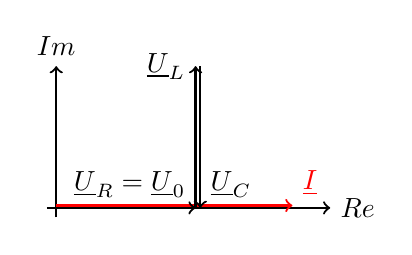
\begin{tikzpicture}[scale=0.6, thick]
	%Koordinatensystem
	\draw[->] (-0.2,0) -- +(right:6) node[right] {$Re$};
	\draw[->] (0,-0.2) -- +(north:3.2) node[above] {$Im$};
	
	%Pfeile
	\draw[->, color=red] (0,0.05) -- +(right:5) node[above right]
	{$\underline{I}$};
	\draw[->] (0,0) -- +(right:2.95) node[above left] {$\underline{U}_R
	= \underline{U}_0$};
	\draw[->] (2.95,0) -- (2.95,3) node[left]
	{$\underline{U}_L$};
	\draw[->]	(3.05,3) -- (3.05,0) node[above right]
	{$\underline{U}_C$};

\end{tikzpicture}

